%\section{Asynchronous Programming}
%The core idea of asynchronous programming is to handle all the tasks that need
%to block waiting for results asynchronously, so that nothing is really blocked.

%It can be implemented using an active poll loop. The active poll loop polls
%different event source for events. Whenever an event happens, the poll loop
%executes a callback function associated with the event to handle the event.

%An improved asynchronous programming style is to use futures and promises. The
%future and promise abstraction can handle asynchronous programming in a nice
%manner.

%Asynchronous programming is the solution for all the problems that I have
%mentioned in the previous section.

%\section{Seastar and OSv}

%Seastar is a modern asynchronous programming library with future and promise
%style. It can be combined together with DPDK to achieve low-level packets
%processing. It also includes a user-space TCP/IP stack that is driven by
%asynchronous programming.

%It is the best asynchronous programming library that we can use to build network
%functions.

%Seastar can also run in OSv, a unikernel. In this way we can achieve
%high-performance virtualization.

%\section{Planned Roadmap}

%I plan to do the following case studies using Seastar in this work.

%First, implementing an unified NFV platform like NetBricks. Highlight that with
%the help of C++ unique\_ptrs, we can achieve the similar software memory safety
%like NetBricks.

%Second, port PRADS to use Seastar. Show that with the help of asynchronous
%programming, we can greatly improve the performance of PRADS.

%Third, implement a simplified version of mOS. Show that asynchronous programming
%can greatly simplify flow event generation and processing.

%Fourth, re-implement FTMB. Show that how easy it is to implement primary-backup
%replication for network functions using seastar.

%Fifth, a simplified SDN switch using Seastar, show it's performance boost when
%compared against OpenVSwitch.

\section{Promises and Cooperative Threads}

In this section, I will first give a detailed overview about promises and
cooperative threads used by Seastar fraemwork. Then I will introduce how to
apply promises and coopeartive threads to NFV.

\subsection{Lwt}

The core building blocks of Seastar are promises and cooperative
threads. Clearly, these fancy concepts come from the world of functional
programming languages. There is an Ocaml library called Lwt \cite{vouillon2008lwt}, which also
implements promises and cooperative threads. In the following sections, I will
first discuss how promises and coopeartive threads are implemented in
Ocaml. Then I will show how they are implemented in Seastar.

\subsubsection{Lwt Overview}

When wring programs like network servers, non-blocking is a very important
property that ensures the runtime efficiency of the network servers. There are
two dominant techniques to make the program non-blocking. The first one uses
multi-threading to support non-blocking, i.e. whenever a blocking operation is
going to be made, the main thread of the program lanuches another thread to
handle the blocking operation. The second one uses event-based programming
method, i.e. the main thread treats the completion of the blocking operation as
an event and register corresponding event handlers to handle this event.

The first technique is easy to use and easy to program. The program can be
written in traditonal way without relying on callbacks. However, the first
technique lacks efficiency, as launching too many threads compromises the
runtime performance. On the other hand, the second technique has superior
runtime performance, as it only maintains a single thread. However, it is
difficult to write programs using the second technique due to excessive use of
callbacks.

Lwt uses promises and cooperative threads to support non-blocking. The runtime
performance of Lwt is very good, as it only maintains a single physical thread
like the second technique. And it is quite easy to use. Writing asynchrounous,
fully non-blocking programs using Lwt is just like writing synchronous, blocking
programs using the first technique.

%\verb!sdfs\_dff!

%\begin{verbatim}
%Text enclosed inside environment
%is printed directly
%and all \LaTeX{} commands are ignored.
%\end{verbatim}

In the following sections, to facilitate understanding, I simplify some concepts
related with exception handling and modify the name of some important types in
Lwt.

\subsubsection{Promise State}

\begin{figure}[!h]
        \centering
        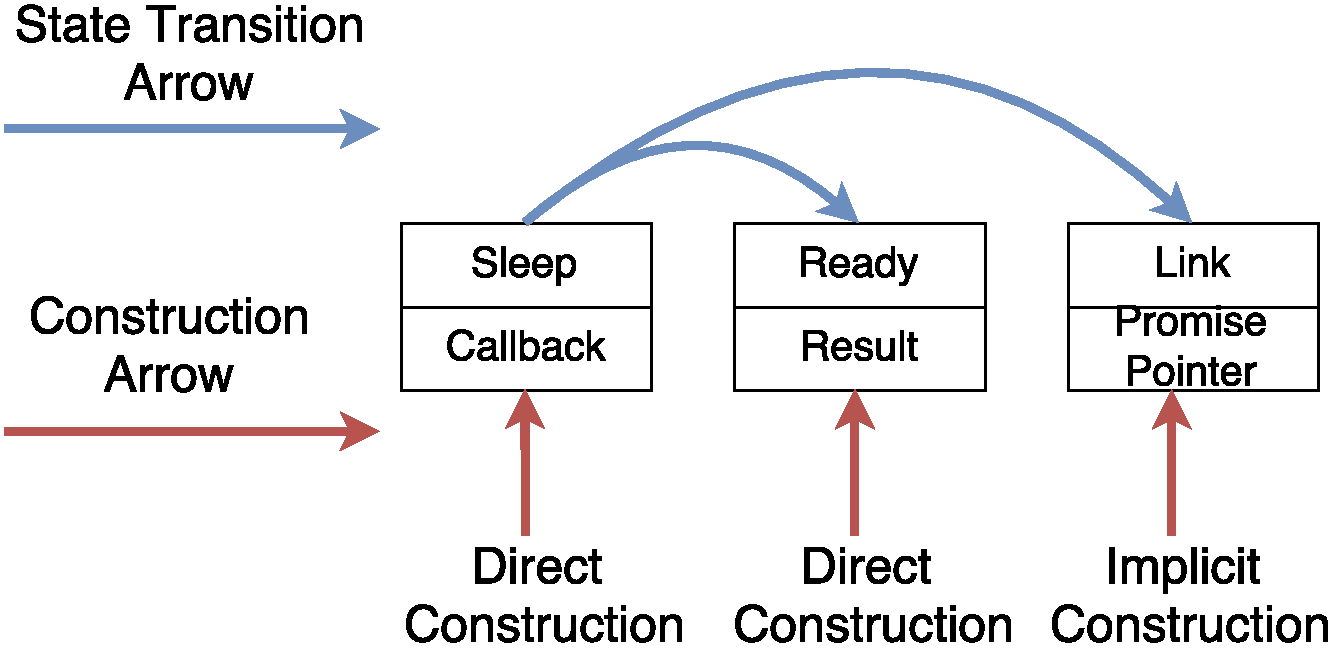
\includegraphics[width=1\columnwidth]{figure/promise-state.pdf}
        \caption{The state of a promise. The blue arrow represents how future
          states are transitioned. The red arrow represens whether can a
          programmer construct a certain state.}
        \label{fig:promise-state}
\end{figure}

The basic building block in Lwt is promise. A promise, as shown in figure
\ref{fig:promise-state}, has three states, which are \textbf{Sleep} state,
\textbf{Ready} state and \textbf{Link} state. The \textbf{Sleep} state
represents that the result of the promise is not available yet and one has to
wait before the \textbf{Sleep} state transitions into \textbf{Ready} state. The
\textbf{Sleep} state promise may contain a callback function, which is
immediately called after it is transitioned to \textbf{Ready}
state. \textbf{Ready} state represents that the result is available and we can
peek the result by checking the result field. Finally, the \textbf{Link} state
contains a pointer to a promise that is in \textbf{Sleep} state. It is used to
when waiting for multiple events.

The state of a proimse can be changed. The blue arrow of figure
\ref{fig:promise-state} shows the state transition graph between the three
states. Only \textbf{Sleep} state can generate a state transition.

When programming with promises, the programmer can only construct \textbf{Sleep}
state promise and \textbf{Ready} state promise. The \textbf{Link} state promise
is implicited constructed when chaining a promise with an annoynamous function
(we omit the discussion, as it does not affect the understanding of how promises
work).

\subsubsection{Chaining Promises}

\begin{verbbox}(>>=) : Promise a -> (a -> Promise b) -> Promise b \end{verbbox}

\begin{figure}[!h]
\resizebox{0.95\columnwidth}{!}{\theverbbox}
\caption{The infix operator for chaining promises.}
\label{fig:infix}
\end{figure}



Multiple promises can be chained together to accomplish complicated
tasks. Chaining is done through an infix operator \verb!>>=! (the then member
function of future in Seastar) as shown in figure \ref{fig:infix}, whose
signature is listed below.

Here, \verb!Promise a! represents a promise that, when transitioning into
\textbf{Ready} state, contains a result field with type \verb!a!. \verb!(a -> Promise b)!
represents an annouymous function, that takes a value of type \verb!a! as
argument and returns a value with type \verb!Promise b!. \verb!>>=! is a
function, that takes a value of \verb!Promise a! and an anouymous function of
\verb!(a -> Promise b)! and returns a value of \verb!Promise b!.

The real power of the \verb!>>=! operator is to chain multiple promises together
into a complicated operation. We give a piece of example code in figure
\ref{fig:example}. The code will first sleep for 3 seconds, then print "first
print" on the screen, then sleep another 3 seconds, and finally print "second
print" on the scrren. The best thing about this code is that, even if it
represents the consecutive execution of four blocking operations, but the code
itself is not blocking at all. It will return a promise in \textbf{Sleep} state
after being called. The blocking operations are implicitly handled by a
background thread.

\begin{verbbox}
  sleep 3 >>=
  fun () -> async_print "first print" >>=
  fun () -> sleep 3 >>=
  fun () -> async_print "second print"
\end{verbbox}

\begin{figure}[!h]
\resizebox{0.95\columnwidth}{!}{\theverbbox}
\caption{Chaining multiple promises into a complicated operation. The code above
  will first sleep for 3 seconds, then print "first print" on the screen, then
  sleep another 3 seconds, and finally print "second print" on the scrren.} 
\label{fig:example}
\end{figure}

\subsubsection{Annatomy of the infix operator}

\begin{verbbox}
(>>=) x f =
  match x with
  | Result r -> f r
  | Sleep ->
    let res = make_Sleep_promise () in
    add_callback x ( fun x -> connect res (x >>= f) )
    res
  | Link p ->
    assert false

connect t t' =
  match t' with
  | Result r -> (run t's callback)
  | Sleep ->
    (let t' link to t)
  
\end{verbbox}
\begin{figure}[!h]
\resizebox{0.95\columnwidth}{!}{\theverbbox}
\caption{The implementation of the infix operator. } %Depending on the state of the
  %promise \verb!x!, \verb!>>=! steps into three branches. If \verb!x! is a
 %result promise, then the annoynamous function.}
\label{fig:infix-internal}
\end{figure}

\noindent \textbf{The internal of the infix operator.} Depending on the state of
promise \verb!x!, the infix operator may step into two branches. If \verb!x! is
in \textbf{Result} state, then the anonymous function is immediately
excuted. But if \verb!x! is in \textbf{Sleep} state, the operator first creates a new
promise \verb!res! in \textbf{Sleep} state. Then a callback is added to \verb!x!. When
\verb!x! becomes \textbf{Result} state, the callback function is called, which
connects \verb!res! and \verb!x >> f!. The \verb!connect! function means that
the state of promise \verb!t'! will be reflected in promise \verb!t!.

\noindent \textbf{A conceptual explanation.} When executing \verb!x >>= f!, if
\verb!x! is immediately available and in \textbf{Result} state, then the
execution of the anonymous function \verb!f! continues without any
interruption.

The tricky part comes when \verb!x! is in \textbf{Sleep} state. It implies that
the result of \verb!x! is going to be available in the future. To prevent the
infix operator from blocking, we construct a new \textbf{Sleep} state promise
\verb!res! and returns \verb!res! to the user. Apparently, \verb!res! should
reflect the actual result of \verb!x >>= f!. To achieve this, before returning
\verb!res! to the user, we add a callback function to \verb!x!, which manually
connect \verb!res! with \verb!x >>= f! when \verb!x! becomes ready. In this way,
we mannualy construct a fully non-blocking abstraction.


\subsubsection{Wake Up Sleep Promise}

If a promise is in \textbf{Sleep} state, it must be waken up in the future and
transform into \textbf{Result} state. This is done by an external polling thread
which polls asynchronous completion messages. If the blocking operation that a
\textbf{Sleep} promise waits for has completed, the corresponding promise is
waken up.

\subsection{Seastar}

Seastar is basically a re-implementation of lwt in C++. It differes from lwt:

\textit{First}, the infix operator \verb!>>=! that chains promises together becomes
\verb!then! member function.

\textit{Second}, Seastar introduces a new object called \verb!future!, which is actually
a pointer object to the underlying promise. The reason is that C++ has no
garbage collection and Seastar has to manually manage the the memory allocation
of the promise object. Currently, Seastar either allocates the promise object
directly on the heap, or captures the promise object inside the callback
function. Therefore, to query the promise, seastar creates a pointer object
future, which contains a pointer to the underlying promise object.


\subsection{Promises in NFV}

We use promises to hide any kind of blocking operations when processing
packets. We give some usage examples.

\subsubsection{Simple Packet Processing}

\begin{verbbox}
xxx.then([]{
  process packet;
  return new_future;
}).then([]{
  process packet;
  return new_future;
})
  
\end{verbbox}
\begin{figure}[!h]
\resizebox{0.5\columnwidth}{!}{\theverbbox}
\caption{Example code of a simple packet processing software.} 
\label{fig:spps}
\end{figure}

It is straightforward to implement a simple packet processing software using
promises, as shown in figure~\ref{fig:spps}. The multiple chained promises
represent multiple processing stages on a packet processing pipeline.

\subsubsection{Using Promises to Hide Blocking During File IO}

\begin{verbbox}
xxx.then([]{
  do file IO;
  return new_future;
}).then([]{
  resume packet processing;
  return new_future;
})
  
\end{verbbox}
\begin{figure}[!h]
\resizebox{0.5\columnwidth}{!}{\theverbbox}
\caption{Example code of a NF that performs file IO.} 
\label{fig:file-io}
\end{figure}

Figure \ref{fig:file-io} represents a NF that performs file IO in the middle of
packet processing. Previously, this incurs kernel context switches and blocking,
which may compromise the performance of the NF. But with promise, the kernel
context switches and blocking are hidden by the promises, making the entire
operation fully non-blocking.

After issuing \verb!do file IO!, the NF software can continue to process other
flows. When file IO finishes, the processing of the original packet that incur
the file IO is resumed. This can greatly boost the performance of NFs that need
to perform file IO, such as PRADs.

\subsubsection{Handling Shared Variable Accessing}

\begin{verbbox}
xxx.then([]{
  access shared variable;
  return new_future;
}).then([]{
  resume packet processing;
  return new_future;
})
  
\end{verbbox}
\begin{figure}[!h]
\resizebox{0.5\columnwidth}{!}{\theverbbox}
\caption{Example code of a NF that needs to access shared variable.} 
\label{fig:asv}
\end{figure}

Figure \ref{fig:asv} shows an example of how to use promise to handle shared
variable processing. After issuing \verb!access shared variable!, the processing
is temporarily suspended and a request is created and sent to another thread to
access the shared variable. After modifying the shared variable, the suspended
packet processing is resumed.

By using promises, we can effectively linearize shared variable
accessing. Therefore we can keep the primary NF instance and the backup NF
instance in the same state, which simplifies primary-backup replication even in
multi-threaded environment.

